\chapter{Reproducing kernel Hilbert space (RKHS) for learning}
\label{ch:rkhs}
The standard LSTD and $\gradTD$ learning algorithms were discussed in \Chapter{ch:diff_td}. One of the important steps in both these algorithms is the selection of a suitable approximating function class, characterized by  a linear or nonlinear parameterization. It is noted in \cite{ctcn} that any insight about the true value function can aid in this step. For example, if the value function is known to obey certain properties, say convexity, then the basis functions chosen can also be convex. In the case of stochastic optimal control, the \textit{fluid} value functions provide a natural starting point to approximate the solution to the average-cost value function. However, such choices are heavily problem-dependent and no standard methods exist In most traditional examples of TD learning, a predetermined set of basis functions is used to define the function class. This limits the learning problem in two ways:
\begin{itemize}
	\item The chosen function class may not be rich enough to give a good approximation of the value function.
	\item Additionally, the approximation algorithms discussed in this thesis are based on Monte Carlo methods with finite sample size. A predetermined set of basis functions will not be able to exploit information about the distribution of these samples.  
\end{itemize}
Hence, it seems better to choose a function class that adapts dynamically to suit the problem and the sample distribution. Kernel methods provide an alternative approach to basis selection. 

In this chapter, the $\gradTD$ algorithm that was proposed in \Chapter{ch:diff_td} is adapted to work in a reproducing kernel Hilbert space (RKHS) setting.  The remainder of this chapter is organized as follows - In \Section{s:rkhs_basics}, a very concise introduction to kernel functions and the RKHS theory is provided. We discuss some properties of the RKHS associated with the Gaussian kernel, that make them \anand{universal} widely used in \Section{s:gaussian_rkhs}. A short review of the various existing approaches to error analysis for a generic least squares regression problem is given in \Section{s:erm_error}. The problem of approximating the gradient of the solution to Poisson's equation \eqref{e:gradTD_norm_error} is reformulated as an empirical risk minimization (ERM) in \Section{s:erm} and a solution is obtained using a general version of the representer theorem in \Section{s:rep_theorem}.  Error analysis for the case of loss functions with gradient terms, which is relevant to the problem discussed in this thesis in \Section{}
 
\section{RKHS Basics}
\label{s:rkhs_basics}
Reproducing kernel Hilbert spaces (RKHS) have been quite well-studied for over five decades now. Their mathematical properties were first studied by Moore \cite{moo1916}, Aroszajn \cite{aro50} etc. Although initial applications were in time series, detection, filtering and prediction problems, more recently they have been found to be incredibly useful in machine learning \cite{wah90}. With the development of support vector machine (SVM) for classification and regression problems \cite{corvap95, drucburkaufsmovap97}, kernel methods have gained a lot of popularity in the machine learning community. 

In this thesis, kernel methods and RKHS are employed with the objective of learning functions from observed data. Such class of problems termed \textit{empirical risk minimization} (ERM) also have a rich history in statistical learning theory. The key objective in such problems is not just to obtain a good fit on the observed data, but to generalize well on ``unseen'' data as well. Regularization methods are used to prevent \textit{overfitting} and achieve better generalization. We consider a Tikhonov regularization scheme \cite{tikars79} associated with \textit{Mercer kernels}.

\subsection{Reproducing kernels} 
Before defining an RKHS, a positive definite kernel needs to be defined. A function $\Kern : X \times X \to \Re$ which for all $N \in \mathbb{N}$ and all $x_1,x_2,\cdots,x_N \in X$ gives rise to a positive definite Gram matrix is a called a positive definite kernel. That is, given any set of points $\{x_i\}_{i=1}^N$, the $N\times N $ matrix whose $ij^{th}$ element $\gram_{i,j} = \Kern(x_i,x_j)$ is positive definite.  

Also defined is $\featuremap: X \to \Re^X$, a feature map that maps each point from $X$ into a function mapping $X$ to $\Re$. Here $\Re^X \eqdef \{f: X \to \Re \}$. One such mapping, called the \textit{canonical} feature map is $\featuremap(x) = \Kern(x,\cdot)$. An inner product is defined such that for all $x,x' \in X$, we have
\begin{equation}
\begin{aligned}
\Kern(x,x') &= \langle \featuremap(x), \featuremap(x')\rangle \\
& = \langle \Kern(x,\cdot), \Kern(x',\cdot)\rangle
\end{aligned}
\label{e:rkhs_inner_product}
\end{equation}
The symmetry of the kernel $\Kern$ follows from the commutative property of the inner product, i.e.,
\[
\Kern(x,x') = \langle \Kern(x, \cdot), \Kern(x',\cdot) \rangle = \langle \Kern(x',\cdot), \Kern(x,\cdot) \rangle = \Kern(x', x). 
\]
Let us consider a function $f$ which is a linear combination of the form,
\begin{equation}
f(\cdot) = \sum_{i=1}^N \alpha_i \Kern(x_i, \cdot),
\label{e:f_rkhs}
\end{equation}
where $N \in \mathbb{N}, \alpha_i \in \Re, x_1,x_2,\cdots, x_N \in X$ are arbitrary. Let $\clH^0$ denote the vector space (pre-Hilbert space) spanned by all functions $f$ of this form. 
The reproducing property of the kernel $\Kern$ follows from the definition of the inner product,
\[
\langle \Kern(x,\cdot), f(\cdot)\rangle = f(x) \qquad \forall x \in X, \forall f \in \clH^0.
\]
Owing to this property, the kernel function $\Kern$ is called the \textit{reproducing kernel}. 

The space obtained by the completion of functions of the form $f$ defined in \eqref{e:f_rkhs}, that are endowed with the inner product as in \eqref{e:rkhs_inner_product} (denoted as $\langle \cdot, \cdot \rangle_{\clH}$ here onward) yields a Hilbert space $\clH$, called the reproducing kernel Hilbert space (RKHS). The corresponding norm is defined as $\|f\|_\clH \eqdef \sqrt{\langle f, f \rangle_\clH}$. The reproducing kernel Hilbert spaces have the remarkable property that norm convergence implies pointwise convergence. 
For any function $f\in\clH$ and $\{f_n\}\subset \clH$ be a sequence with $\|f_n - f\|_\clH \to 0$ for $n \to \infty$, then for all $x \in X$, we have,
\[
\lim_{n\to\infty} f_n(x) = \lim_{n \to \infty} \langle \Kern(x,\cdot),  f_n(\cdot) \rangle_\clH = \langle \Kern(x, \cdot), f(\cdot) \rangle_\clH = f(x)
\]
If $\Kern$ is a continuous, symmetric and positive definite kernel satisfying, 
\[
\kappa = \sup_{x \in X} \sqrt{\Kern(x,x)} < \infty,
\]
then, \Prop{prop:RKHS_bounded} holds.

\begin{proposition}
\label{prop:RKHS_bounded}
	If the kernel $\Kern$ is uniformly bounded, then any $f \in \clH$ is also bounded. 
\end{proposition}
\begin{proof}
	If $f \in \clH$, for all $x \in X$,
	\[
	\begin{aligned}
	|f(x)| &= |\langle \Kern(x,\cdot), f \rangle_\clH| \\
	& \leq \|\Kern(x,\cdot)\|_\clH \|f\|_\clH \qquad{\text{(By Cauchy-Schwarz inequality)}}\\ 
	& \leq \kappa \|f\|_\clH
	\end{aligned}
	\]
	As the above inequality holds for all $x \in X$, 
	\[
	\|f\|_\infty := \max_{x\in X}|f(x)| \leq \kappa \|f\|_\clH
	\]
\end{proof}
A Hilbert function space $\clH$ that has a reproducing kernel $\Kern$ is always an RKHS and conversely, every RKHS has a (unique) reproducing kernel. However, the feature map $\featuremap$ is non-unique. 
\subsection{Orthonormal basis functions} \anand{Mercer's theorem?}
Given $\clH$, it is of interest to understand the basis functions that span the Hilbert space. This can be studied using Mercer's theorem \cite{merrus09}.
Consider the integral operator (Hilbert-Schmidt operator) $L_K:L^2_\measure(x) \to L^2_\measure(x)$ defined by,
\[
(L_K f)(x) = \int_X \Kern(x,t) f(t) d\measure(t)
\]
where $\measure$ is a finite Borel measure and $X$ is a compact set.
The linear map $L_K^{1/2}$ is a Hilbert isomorphism between $L^2_{\measure}(X)$ and $\clH$ as illustrated in \Fig{fig:rkhs_isomorphism}. 

\begin{figure}[htbp]
	\centering
	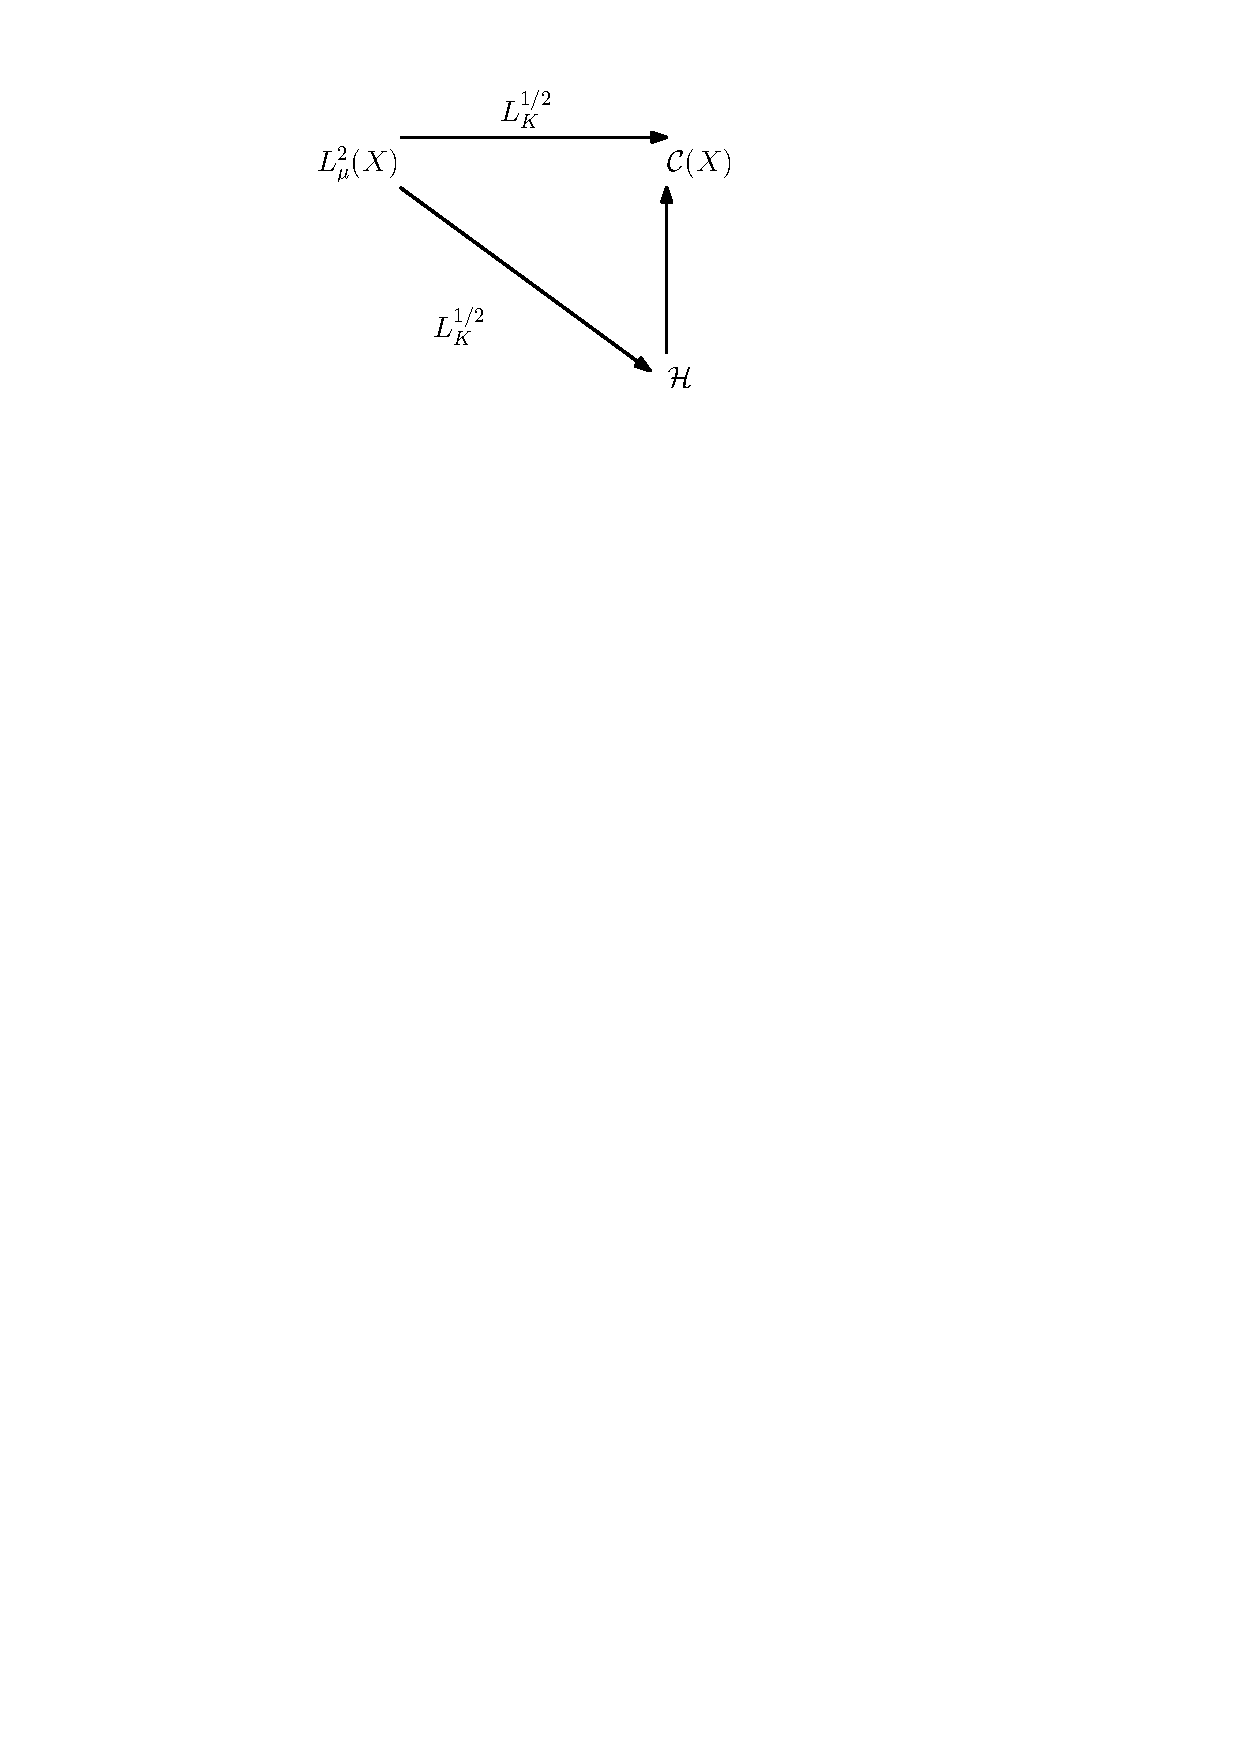
\includegraphics[width=3in]{images/Chap3_RKHS_isomorphism}
	\caption{Diagram illustrating the isomorphic transformations between $\clH$ and $L^2_\measure$.}
	\label{fig:rkhs_isomorphism}
\end{figure}

% $L_{K,C}$ emphasizes that the target is $\mathcal{C}(X)$ and $I_K$ denotes the inclusion. If $\Kern$ is $\mathcal{C}^\infty$, then $I_K$ is compact. \anand{Gaussian kernel is $\mathcal{C}^\infty$}
 $L_K$ is a self-adjoint, compact operator with eigenvalues $\reg_1 \geq \reg_2 \geq \cdots \geq 0$, with the corresponding normalized eigenfunctions $\{\phi_n\}_{n=1}^\infty$ forming an orthonormal basis for $L^2_\measure(X)$. Mercer's theorem states that 
\[
\Kern(x,t) = \sum_{n=0}^\infty \reg_n \phi_n(x) \phi_n(t)
\]
where the series converges absolutely for each $x,t \in X$. The set $\{\sqrt{\reg_n}\phi_n\}_{n=1}^\infty$ forms an orthonormal basis for $\clH$. 


\section{Properties of the Gaussian kernel -  RKHS}
\label{s:gaussian_rkhs}

Of the many kernels being used, Gaussian kernel is the most widely used and often gives the best performance. The study of the properties of the Gaussan kernel has received a lot of attention \cite{stehussco06, min10}. The Gaussian kernel for $X = \Re^d$ is given by,
\[
\Kern_{\epsilon}(x,x') := \exp(-\|x - x'\|^2/ 4\epsilon) \qquad \forall x,x' \in \Re^d
\]

\begin{figure}[htbp]
	\centering
	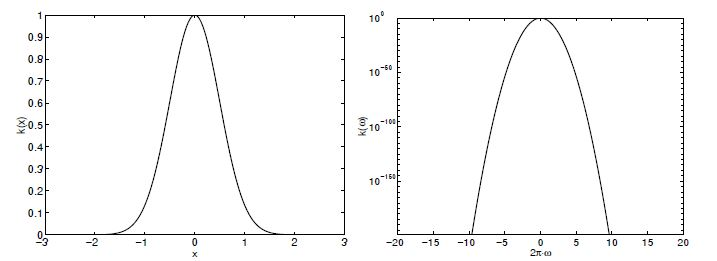
\includegraphics[width=5in]{images/Chap3_Gaussian_kernel}
	\caption{Gaussian kernel with $\epsilon = 0.125$ and its Fourier transform \cite{schsmo01}.}
	\label{fig:gaussian_kernel}
\end{figure}

This paper tries to answer questions like - which functions are contained in the RKHSs induced by the Gaussian kernel, how the corresponding norms can be computed, and how the RKHSs of different widths correlate to each other. 
In particular, RKHSs of Gaussian kernels always have countable orthonormal bases. 

Theorem 3 of the paper gives the orthonormal basis functions for $\clH$ defined the Gaussian kernel $\Kern_\epsilon$. It states that for $\epsilon >0$ and $n \in \mathbb{N}_0 := \mathbb{N} \cup \{0\}$, we define the function $\phi_n : \Re \to \Re$ by
\[
\phi_n(x) := \sqrt{\frac{1}{(2\epsilon)^n n!}}x^n \exp(-x^2/4\epsilon)
\]


The paper gives several properties of the reproducing kernel Hilbert space induced by the Gaussian kernel \cite{min10}.
Theorem 1 of the paper states that the RKHS $\clH$ induced by the standard Gaussian kernel is infinite dimensional, i.e. dim($\clH$) = $\infty$ and 
\[
\clH := \Bigl\{ f = \exp(-x^2/4\epsilon) \sum_{n=0}^\infty w_n x^n: \|f\|^2_\clH = \sum_{k=0}^\infty (2\epsilon)^k k! \sum_{n=0}^k w_n^2 <\infty \Bigr\}
\]
The paper presents the orthonormal basis for $\clH$ which is consistent with the expression in the previous reference. 

\begin{enumerate}
	\item $\clH$ induced by the standard Gaussian kernel does not contain any polynomial on $X$, including the non-zero constant function. 
	
	\item If $X$ is compact, $\clH$ induced by the Gaussian kernel is dense in the space of $\mathcal{C}(X)$ of continuous functions on $X$.
	This means that given a continuous function $h(x)$, for all $\varepsilon >0$, we can find a function $g(x) \in \clH$ such that 
	\[
	\|h(x) - g(x)\|_\infty \leq \epsilon \qquad \forall x \in X
	\] 
	\item Let $\Kern_{\epsilon}(x,y) = \exp(-\frac{\|x-y\|^2}{4\epsilon})$. The Hilbert space $\clH$ induced by $\Kern_\epsilon$ on $X$ contains the function $\exp(-\frac{\mu \|x\|^2} {4 \epsilon})$ if and only if $0<\mu <2$. For example, $\exp(-\frac{\|x\|^2}{2 \epsilon}) \in \clH_{\epsilon/2}$, but  $\exp(-\frac{\|x\|^2}{2 \epsilon}) \notin \clH_{\epsilon}$.
	
	\item The functions in $\clH$ that are smooth are not necessarily integrable, as $\clH \notin L^1(\Re^n)$ for any $\epsilon >0$. 
	

\item Partial derivatives of the Gaussian kernel denoted as $D^\alpha \Kern_x \in \clH$. As a corollary, it can be shown that $t^\alpha \Kern_x(t)\in\clH$. Additionally, for any polynomial $p(t)$, $p(t) \Kern_x(t) \in \clH$. 

\end{enumerate}

\textbf{Implications for learning theory and function approximation}

$L^1$ norm optimization or regularization is infeasible in $\clH$. This could still be done on subsets of finite linear combinations of the basis functions.

The paper also provides the expression for the Hilbert space norm for kernel derivative of any order $d$. 

\cite{micchaxuzha06}
This paper sets out to identify kernels with \textit{universal approximating property} - Given any compact set $X$,  any positive number $\varepsilon$ and any function $f \in \mathcal{C}(X)$, there is a function $g \in \clH$ such that $\| f - g\|_{\infty} \leq \varepsilon$. Thus for any choice of compact set $X$, the set $\Kern(X)$ is dense in $\mathcal{C}(X)$ in the maximum norm. A kernel that satisfies this property is called the \textit{universal kernel}. The paper discusses the characterization of universal kernels in terms of feature map representation of the kernel $\Kern$. It provides necessary and sufficient condition for $\Kern$ to have the universal approximation property in terms of its features. 

As a consequence of Theorem 17 of the paper, the standard Gaussian kernel is shown to be universal. 


An interesting question in the context of FPF gain function approximation would be whether the following holds true for a sequence of functions $\{g_n\} \subset \clH$.
\begin{enumerate}
\item $\lim_{n \to \infty} \sup_x |g_n(x) -h(x) | \to 0,\quad \forall x \in \Re$
\item $ \lim_{n \to \infty}\sup_{x \in X} |g_n(x) - h(x) | \to 0$ and $\sup_x |g_n(x)| < \infty,  \forall x \in \Re$ and $X$ is a compact subset of $\Re$. 
\end{enumerate}
This ensures that the gain approximation $g_n$ is arbitrarily close to the true gain within a compact set $X$ and it does not become unbounded anywhere. 


\section{Error Analysis}
\label{s:erm_error}
Although ideally, we would like to obtain the best \textit{target} function often called the \textit{regression} function, practically this is not possible due to the choice of the approximating function space and the fact that only a finite number of data points are available. Error arising from the former is termed \textit{approximation error} and the latter is termed \textit{sample error}. A wide variety of literature exists on error analysis. Bounds for the approximation error have been studied from various perspectives - i) methods based on complexity of the hypothesis space (like VC-dimension \cite{gir95}, covering numbers \cite{zhou02, smazhou03, zhou03}), ii) methods based on \textit{stability} of the learning algorithm \cite{boueli01,boueli02}.

In general, the goal of a learning problem is to find an approximation of a function $f_\pr : X \to Y$, when only a pair of values $z = (x_i, y_i)_{i=1}^N$ drawn from an unknown probability measure $\pr$ on $X \times Y$ is available. A common approach followed is to minimize,
\[
f_{\reg,z} := \argmin_f \frac{1}{N}\sum_{i=1}^N (f(x_i) - y_i)^2 + \reg \|A f \|^2_{\mathcal{L}_{\pr}^2(X)}
\]
where $A$ is an operator and $\mathcal{L}^2_{\pr}(X)$ is the Hilbert space of square integrable functions on $X$ with measure $\pr_X$ on $X$. Here, $f_\pr$ is the ``regression'' function of $\pr$,
\begin{equation}
f_\pr(x) = \int_Y y d\pr(y|x)
\label{eq:f_rho}
\end{equation}

References
\begin{itemize}
\item Best choices of regularization parameters in Learning theory - On the bias-variance problem, 2002 by Felipe Cucker, Steve Smale


The main result in this work states that for each $N\in \mathbb{N}$ and $\delta \in [0,1)$, a function $E_{N,\delta} = E : \Re_+ \to \Re$ exists such that for all $\reg >0$,
\[
\int_X (f_{\reg,z} - f_\pr)^2 \leq E(\reg)
\]
with confidence $1-\delta$. The ``best'' regularization parameter $\reg^*$ depends on the number of samples $N$, confidence interval $1-\delta$ and the operator $A$ and a simple invariant of $\pr$. The assumption is that $f_\pr \in \mathcal{L}^2_\pr(x)$ is bounded. 

The authors construct the two related minimization problems: 
\[
\begin{aligned}
\text{Problem 1 :} \min & \int_X(f(x) - y)^2 + \reg \|f\|^2_\clH, \\
\text{s.t.} & f \in \clH \\
%\end{aligned}
%
%\[
%\begin{aligned}
\text{Problem 2 :} \min & \frac{1}{N} \sum_{i=1}^N (f(x_i) - y_i)^2 + \reg \|f\|^2_\clH,\\
\text{s.t.} & f \in \clH
\end{aligned}
\]
A theorem in the paper states that the minimizers $f_\reg$ and $f_{\reg,z}$ of problems $1$ and $2$ respectively exist, are unique and are given by, 

\[
\begin{aligned}
\text{Solution to problem 1:} &
f_\reg = (I_d + \reg L_\Kern^{-1})^{-1} f_\pr, \\
\text{Solution to problem 2:} & 
f_{\reg,z}(x) = \sum_{i=1}^N \beta_i \Kern(x,x_i)
\end{aligned}
\]
where $\mathbf{\beta}: = [\beta_1, \beta_2, \hdots, \beta_N]$ is the unique solution of the well-posed linear system in $\Re^N$,
\[
(\reg N I_d + \Kern) \mathbf{\beta} = \mathbf{y}
\]
The Hilbert space norm $\|f\|^2_\clH = \beta^\transpose \Kern \beta$.

The paper defines error $\mathcal{E}$ as 
\[
\mathcal{E} = \int_Z (f(x) - y)^2
\]
and empirical error $\mathcal{E}_z$ given a sample $z \in Z_N$ as,
\[
\mathcal{E}_z = \frac{1}{N} \sum_{i=1}^N (f(x_i) - y_i)^2
\]
\[
\mathcal{E}(f_{\reg,z}) = \mathcal{E}(f_{\reg, z }) - \mathcal{E}(f_\reg) + \mathcal{E}(f_\reg)
\]
Therefore, 
\[
\mathcal{E}(f_{\reg,z}) \leq \underbrace{|\mathcal{E}(f_{\reg,z}) - \mathcal{E}(f_\reg)|}_{\text{sample error}} + \underbrace{\mathcal{E}(f_\reg)}_{\text{approximation error}}
\]

\noindent \textbf{Sample Error :}
Theorem 2 in the paper gives probabilistic bounds for the \textit{sample error}.
Theorem 3 states that given $N>0$, $0<\delta \leq 1$, and for all $\reg>0$, the expression 
\[
\mathcal{S}(\reg) = \frac{32 M^2 (\reg + C_K)^2}{\reg^2} v^*(N,\delta)
\]
where $M$ and $C_K$ are appropriate constants defined in the paper. 

\noindent \textbf{Approximation Error :} To choose the optimal $\reg$, the paper looks at the \textit{approximation error}. 
\[
\min_{f \in \mathcal{L}_\pr^2(X)} (\|f - f_\pr\|^2 + \reg \|f\|^2_\clH) \leq \reg^\theta \|L_K^{-\theta/2} f_\pr \|^2
\]
The minimum is obtained for $f = f_\reg$. Therefore,
\[
(\|f_\reg - f_\pr\|^2 + \reg \|f_\reg\|^2_\clH) \leq \reg^\theta \|L_K^{-\theta/2} f_\pr \|^2
\]
A basic result in Chapter 1 of CS states that for all $f_\pr \in \mathcal{L}_\pr^2(X)$, 
\[
\mathcal{E}(f) = \int_X (f - f_\pr)^2 + \sigma_\pr^2
\]
where $\sigma_\pr$ depends only on $\pr$. Therefore, approximation error $\mathcal{E}(f_\reg)$ is bounded by,
\[
\begin{aligned}
\mathcal{E}(f_\reg)  & \leq \reg^\theta \|L_K^{-\theta/2} f_\pr \|^2 + \sigma_\pr^2\\
& \leq \mathcal{A}(\reg) + \sigma_\pr^2 
\end{aligned}
\]

Now, let $E(\reg) = \mathcal{S}(\reg) + \mathcal{A}(\reg)$. 
Recall,
\[
\begin{aligned}
\mathcal{E}(f_{\reg,z}) &\leq |\mathcal{E}(f_\reg) - \mathcal{E}(f_{\reg,z})| + \mathcal{E}(f_\reg) \\
& \leq \mathcal{S}(\reg) + \mathcal{A}(\reg) + \sigma_\pr^2\\
& \leq E(\reg) + \sigma_\pr^2
\end{aligned}
\]
Subtracting $\sigma_\pr^2$ from both sides, we get
\[
\int_X (f_{\reg,z} - f_\pr)^2 \leq E(\reg)
\]

The optimal $\reg^*$ that minimizes both the sample error and the approximation error can be obtained by taking the derivatives with respect to $\reg$ and equating $\mathcal{S}'(\reg^*) + \mathcal{A}'(\reg^*) =0$. Corollary 2 also gives that for every $0 <\delta \leq 1$, 
\[
\lim_{N \to \infty} E(\reg^*) = 0 
\]
It has been stated that $\reg^* \to 0$ as $N \to \infty$.

The paper concludes with some discussion about the \textit{bias-variance} problem. Roughly speaking, the ``bias'' of a problem coincides with the approximation error and the ``variance'' with the sample error. The bias-variance trade-off amounts to the choice of a compact subspace $\clH$ of $\mathcal{C}(X)$ over which $\mathcal{E}_z$ is minimized. A small subspace $\clH$ will result in a large bias, whereas too much flexibility of $\clH$ for a given dataset $Z$ will produce a large variance. 
Several parameters(radius of balls, dimensions etc.) determine the ``size'' of this subspace $\clH$. For example, if we consider the ball of radius $r = \|f_{\reg,z}\|_K$ in $\clH_K$ and $\clH = \overline{I_K(B_r)}$. Since $\reg \propto \frac{1}{r}$, large $\reg$ corresponds to large bias or approximation error and small $\reg$ corresponds to large variance or sample error. 

\item Support vector machine soft margin classifiers - Error Analysis, 2004

In Zhang (2004) the leave-one-out technique was applied to improve the sample error estimates given in Bousquet and Ellisseeff (2002): the sample error has a kernel-independent bound $O(\frac{C}{N})$,
improving the bound $O(\frac{C}{\sqrt{N}})$ in Bousquet and Ellisseeff (2002).

This paper mostly considers the soft SVM classifier. It does not say anything about the least squares error.

\item Stability and Generalization, 2002 - Bousquet and Elisseeff

In this work, the accuracy of learning algorithms is analyzed using a different approach based on \textit{sensitivity analysis}. Sensitivity analysis aims at determining how much the variation of the input can influence the output of the system. The difference between an empirical measure of error and the true generalization error is taken as a random variable. This paper introduces three notions of stability and then derives bounds on the generalization error of stable learning systems. Many algorithms including regularized least squares regression in an RKHS satisfies the stability requirements.

General discussion -  When trying to estimate an unknown function from data, one needs to find a tradeoff between bias and variance. One approach is to keep increasing the size of the model and then choosing the best estimator based on a complexity penalty (regularization term). Another approach is statistical methods like bagging, which consists of averaging several estimators built from subsamples of the data.
This work derives exponential upper bounds on the generalization error based notions of stability. Both the leave-one-out error and the empirical error are considered as possible estimates of the generalization error. 

Section 5.2.2 discusses the application of the results to regularization in Hilbert spaces. Theorem 22 states the uniform stability of a reproducing kernel Hilbert space with kernel $\Kern$ such that $\forall x \in X$, $\Kern(x,x) \leq \kappa^2 < \infty$. The learning algorithm defined by a loss function $l$ that is $\sigma$-admissible, 
\[
\argmin_{g \in \mathcal{F}} \frac{1}{N} \sum_{i=1}^N l(g,z_i) + \reg \|g\|^2_\clH
\]
has uniform stability $\beta$ with respect to $l$ with 
\[
\beta \leq \frac{\sigma^2 \kappa^2}{2 \reg N}
\]
Uniform stability is the strongest notion. The algorithm is stable when the value of $\beta$ decreases $\frac{1}{N}$.
Example 3 discusses the stability of regularized least squares regression for a bounded case. The stability bound for this algorithm is
\[
\beta \leq \frac{2\kappa^2 B^2}{\reg N}
\]
The resulting generalization error bound is 
\[
R \leq R_{emp} + \frac{4 \kappa^2 B^2}{\reg N} + \Bigl(\frac{8 \kappa^2 B^2}{\reg} + 2B \Bigr)\sqrt{\frac{\ln 1/\delta}{2N}}
\]
In general, the bounds on generalization error are of the following type, $ R \leq R_{emp} + O(\frac{1}{\reg \sqrt{N}})$. This means that non-trivial results can be obtained only if $\reg >> \frac{1}{\sqrt{N}}$.
\item \rd{A Leave-one-out Cross Validation Bound for Kernel Methods with Appliations in Learning - Zhang}

\item \rd{Optimal rates for the regularized least squares Algorithm, De Vito}

Theorem 1 of the paper gives the optimal choices for $\reg$ as a function of $N$. 

\item \rd{Model selection for regularized least squares regression, De Vito - 2005}

This paper aims to provide a selection rule for the parameter $\reg$ which is optimal for any number $N$ of examples and provides the desired asymptotic behavior when $N$ goes to $\infty$. A sequence of nested hypothesis spaces can be formed for various values of $\reg$,
\[
\clH_{\reg_1} \subset \clH_{\reg_2} \cdots \subset \clH
\]
where $\reg_1 > \reg_2 > \cdots \reg_n$. $\clH_{\reg_k}$ is the subset of functions in the model space $\clH$ that have \textit{complexity} less than $\frac{1}{\reg_k}$. Complexity of the solution decreases with $\reg$.  

In practice, the parameter $\reg$ is usually chosen through an \textit{a posteriori} procedure such as cross-validation or using a validation set.
We are interested in obtaining \textit{a priori} bounds and rules for selection. 
\[
\reg_{opt} := \argmin_{\reg >0} \Expect_D(I[f_D^\reg]),
\]
where $D$ is the training set. It is further refined by considering the variance $\sigma^2$ also,
\[
\reg_{opt} := \argmin_{\reg >0} \{\Expect_D(I[f_D^\reg])+ \sigma^2(I[f_D^\reg])\}
\]
It also considers the worst case analysis, where given a confidence level $\delta \in (0,1)$, 
\[
\begin{aligned}
E_{opt}(\reg, \delta) &:= \inf_{t \in [0;+\infty)} \{t | \text{Prob}\{D \in Z^N | I[f^\reg_D] >t\}\leq \delta\}\\
\reg_{opt}(\delta) &:= \argmin_{\reg >0} E_{opt}(\reg, \delta)
\end{aligned}
\]
This paper is unique in the sense that it does not make use of any complexity measure on the hypothesis space, like VC-dimension or covering number. Instead, the sample error is bounded only through two simple constants related to the topological properties of $X$ and $Y$. 

Theorem 1 gives bounds on the sample error. With probability at least $1-\delta$,
\[
|R[f_D^\reg] - R[f^\reg]| \leq S(\reg,N,\delta)
\]
where $S(\reg,N,\delta) = \frac{M \kappa^2}{\reg \sqrt{N}}\Bigl( 1 + \frac{\kappa}{\sqrt{\reg}}\Bigr) \Bigl( 1 + \sqrt{2 \log \frac{2}{\delta}}\Bigr)$. Here $M = \sup\{|y|\,|y \in Y\}$.

The best rate convergence is obtained by choosing $ \reg_N = \frac{1}{\sqrt[4]{N}}$. 

\item \rd{Learning theory estimates via integral operators and their approximations, Smale Zhou}
Theorem 5 - Obtains error bounds $\|f_{z,\reg} - f_\pr \|_\pr$ is $O(1/\reg\sqrt{N})$. 
Similar results and conditions on $\reg > \frac{1}{\sqrt{N}}$
\item \rd{Regularization in kernel learning, 2010 - Mendelson and Neeman}


\item \rd{Fast rates for SVMs using Gaussian kernels, 2007 - Steinwart and Scovel}
\end{itemize}